
\section*{Общая характеристика работы}

\newcommand{\actuality}{\underline{\textbf{\actualityTXT}}}
\newcommand{\progress}{\underline{\textbf{\progressTXT}}}
\newcommand{\aim}{\underline{{\textbf\aimTXT}}}
\newcommand{\tasks}{\underline{\textbf{\tasksTXT}}}
\newcommand{\novelty}{\underline{\textbf{\noveltyTXT}}}
\newcommand{\influence}{\underline{\textbf{\influenceTXT}}}
\newcommand{\methods}{\underline{\textbf{\methodsTXT}}}
\newcommand{\defpositions}{\underline{\textbf{\defpositionsTXT}}}
\newcommand{\reliability}{\underline{\textbf{\reliabilityTXT}}}
\newcommand{\probation}{\underline{\textbf{\probationTXT}}}
\newcommand{\contribution}{\underline{\textbf{\contributionTXT}}}
\newcommand{\publications}{\underline{\textbf{\publicationsTXT}}}
\newcommand{\object}{\underline{\textbf{\objectTXT}}}
\newcommand{\subject}{\underline{\textbf{\subjectTXT}}}

%%% Обоснование выбора названия диссертации
Молекулярная газодинамика "--- это динамика газа, построенная на основе кинетической теории.
Под последней обычно понимают теорию неравновесных свойств газа.
Ключевую роль при описании газа играет отношение длины свободного пробега молекул газа \(\ell\)
к характерному размеру течения \(L\) "--- так называемое число Кнудсена \(\Kn=\ell/L\).
В континуальном пределе (\(\Kn\to0\)) обычно используют законы классической гидродинамики,
основанной на модели сплошной среды, и только в случае конечных \(\Kn\)
учитывают молекулярную структуру газа. Таким образом, в литературе можно встретить
разделение на континуальную гидрогазодинамику и динамику разреженного газа.
Однако имеется достаточно широкий круг задач, для которых уравнения Навье"--~Стокса
некорректно описывают поведение газа даже при \(\Kn\to0\).
Поэтому в настоящем исследовании используется термин \emph{молекулярная газовая динамика},
подчёркивая тот факт, что методы и представления кинетической теории используются
как для разреженного газа, так и для его континуального предела.
Этот термин, по-видимому, впервые предложен в 1970 году М.\,Н.~Коганом~\autocite{Kogan1971review},
позже подхвачен Г.~Бёрдом~\autocite{Bird1981} и Ё.~Соне~\autocite{Sone2007}.

{\actuality}
%%% Современные проблемы и вызовы
Становление молекулярной газодинамики можно связать с важными прикладными направлениями,
возникшими в первой половине XX века.
В частности, задача разделения изотопов стала импульсом для развития асимптотической теории
и методов вычисления транспортных коэффициентов на основе кинетической теории.
Динамика разреженного газа выделилась в отдельную науку благодаря активному освоению космоса.
Первые исследования носили в основном экспериментальный характер,
но в XXI веке превалирующую роль играет компьютерное моделирование, что
говорит о зрелости теоретических представлений дисциплины.
Неравновесное состояние газа описывается в общем случае шестимерной функцией распределения,
её эволюция подчиняется уравнению Больцмана.
Входящий в него нелинейный интеграл столкновений представляет собой нелокальный квадратичный оператор,
что создаёт существенные трудности, как для математического, так и численного анализа.
За последние три десятилетия строгая математическая теория пополнилась множеством фундаментальных результатов,
а стремительный рост суперкомпьютерных мощностей, доступных исследователям и инженерам,
спровоцировал системное развитие численных методов.

%%% Прикладные области
На сегодняшний день можно выделить несколько прикладных областей молекулярной газодинамики:
\begin{enumerate}
    \item \emph{Аэрокосмические исследования}.
    Движение аппаратов в верхних слоях атмосферы сопровождаются сильно неравновесными течениями
    и достаточно большими числами Кнудсена.
    \item \emph{Микроэлектромеханические системы} (\emph{МЭМС}).
    Эта относительно молодая отрасль обуславливает основную волну интереса
    к изучению разреженного газа в начале XXI века.
    В таких МЭМС как приводы, микротурбины и газовые хроматографы возникают разреженные течения газа.
    \item \emph{Аэрозоли}.
    Процесс их образования, изменение их дисперсного состава описываются в рамках кинетической теории.
    Аэрозольные реакторы используются среди прочего для производства стекловолокна,
    кремниевых пластин и углеродного волокна.
    Наконец, конечная фаза существования атмосферных загрязнений "--- это также аэрозольные частицы.
    \item \emph{Вакуумные технологии}.
    Моделирование течений газа, когда число Кнудсена значительно меняется в пространственно"=временных масштабах,
    представляет собой особенно трудную задачу, однако современный уровень развития вычислительных средств
    позволяет во многих случаях обходиться без дорогостоящих экспериментальных прототипов.
\end{enumerate}

Таким образом, актуальность данного исследования обусловлена
\begin{itemize}
    \item активным развитием прикладных областей,
    \item потребностью в высокоточных численных методах,
    \item быстрым ростом доступных вычислительных ресурсов.
\end{itemize}

{\object} "--- движение одноатомного газа различной степени разреженности.
В исследовании одновременно изучается два {\subject}:
\begin{itemize}
    \item методы численного и асимптотического анализа,
    \item физические свойства стационарных течений.
\end{itemize}

{\progress}

%%% формальная асимптотическая теория
Формальная асимптотическая теория уравнения Больцмана была заложена с трудах Д.~Гильберта~\autocite{Hilbert1912},
С.~Чепмена~\autocite{Chapman1916}, Д.~Энскога~\autocite{Enskog1917},
позже развита Д.~Барнеттом~\autocite{Burnett1935}, Х.~Грэдом~\autocite{Grad1963a} и Ё.~Соне~\autocite{Sone2002}.
Решение уравнения Больцмана для слаборазреженного газа допускает отделение гидродинамической части
от существенно неравновесных пространственно"=временн\'{ы}х кинетических слоёв.
Большой цикл работ Киотской группы (Ё.~Соне, К.~Аоки, Ш.~Таката, Т.~Овада и др.)
посвящён высокоточному численному анализу кнудсеновского слоя первого~\autocite{Ohwada1989creep, Ohwada1989jump}
и второго порядка~\autocite{Ohwada1992, Takata2015second, Takata2015curvature}
для диффузного отражения и газа твёрдых сфер.
Различные системы гидродинамических уравнений могут быть получены в зависимости от способа асимптотического масштабирования.
В частности, для медленных неизотермических течений справедливы
\emph{уравнения Когана"--~Галкина"--~Фридлендера} (\emph{КГФ})~\autocite{Kogan1976},
содержащие некоторые ненавье"--~стоксовские члены.

%%% численные методы
Огромное множество исследований посвящено численному решению уравнения Больцмана.
Среди них можно выделить три магистральных направления в зависимости от способа аппроксимации
функции распределения скоростей:
\begin{itemize}
    \item \emph{методы прямого статистического моделирования} (\emph{ПСМ})
    строятся на основе некоторого случайного процесса марковского типа,
    способного аппроксимировать больцмановскую динамику;
    \item \emph{методы дискретных скоростей} подразумевают фиксированный набор доступных молекулярных скоростей;
    \item \emph{проекционные методы} используют разложение по базису в определённом функциональном пространстве.
\end{itemize}
Методы ПСМ в силу своей универсальности и простоты нашли широкое применение в прикладных областях,
однако присущие им флуктуации иногда сильно ограничивают точность получаемых результатов.
Проекционные методы, напротив, обладают наилучшим соотношением погрешности к размерности аппроксимационного пространства,
но, как правило, в достаточно узком классе решений.
Оказалось возможным добиться второго порядка точности в рамках метода дискретных скоростей,
однако для этого потребовался длинный исторический путь.

%%% методы дискретных скоростей
Метод дискретных скоростей был впервые использован А.~Нордсиком и Б.~Хиксом~\autocite{Nordsieck1966}.
Для вычисления интеграла столкновения они использовали кубатуры Монте"=Карло
с последующей консервативной коррекцией функции распределения.
В дальнейшем метод дискретных скоростей развивался С.~Йеном~\autocite{Yen1984},
В.\,В.~Аристовым и Ф.\,Г.~Черемисиным~\autocite{Tcheremissine1980}.
Д.~Гольдштейн, Б.~Стёртевант и Дж.~Бродуелл первыми для решения уравнения Больцмана использовали
кинетические модели газа, допускающие столкновения только в дискретном пространстве~\autocite{Goldstein1989}.
А.~Пальчевский, Ж.~Шнайд\'{е}р и А.\,В.~Бобылев показали, что,
несмотря на присущие им \emph{консервативность} и \emph{энтропийность} на микроскопическом уровне\footnote{
    Каждое дискретное столкновение не уменьшает энтропию, сохраняет массу, импульс и кинетическую энергию.},
теоретический порядок сходимости таких моделей к уравнению Больцмана сильно меньше единицы~\autocite{Palczewski1997}.
В.~Панфёров и А.~Гейнц показали, как специальная замена переменных
позволяет улучшить сходимость, но лишь вплоть до первого порядка~\autocite{Panferov2002}.
\emph{Размазывание (mollification) столкновительного процесса} позволяет естественным образом
решить проблему консервативной аппроксимации, избегая решения целочисленных уравнений:
\begin{itemize}
    \item К.~Бюе, С.~Кордье и П.~Дегон продемонстрировали, как с его помощью обеспечить консервативность
    на макроскопическом уровне (для столкновительного оператора целиком)~\autocite{Buet1998};
    \item Х.~Бабовски построил простейшую схему с консервативностью на мезоскопическом уровне
    (для всей столкновительной сферы)~\autocite{Babovsky1998}, его подход позже развил Д.~Гёрш~\autocite{Goersch2002};
    \item Ф.\,Г.~Черемисин предложил новый класс методов, сохраняющих консервативность
    на микроскопическом уровне (для отдельной столкновительной пары)~\autocite{Tcheremissine1997}.
\end{itemize}
Микроскопическая консервативность, достигнутая Ф.\,Г.~Черемисиным, позволяет построить наиболее эффективную
численную схему и может быть интерпретирована как проекционная процедура Петрова"--~Галёркина,
в которой столкновительные инварианты образуют ортогональную оболочку.
Кроме того, специальная процедура интерполяции функции распределения обеспечивает
энтропийность метода~\autocite{Tcheremissine2000}. Поэтому такой метод будем называть
\emph{консервативным проекционно"=интерполяционным методом дискретных скоростей} (\emph{KПИМДС}).

%%% неравномерные сетки в пространстве скоростей
Во многих прикладных задачах эффективная аппроксимация уравнения Больцмана
требует существенно неоднородной дискретизации в скоростном пространстве.
Неравномерные сетки активно используются
как в методах дискретных скоростей~\autocite{Kolobov2011, Morris2012},
так и проекционных~\autocite{Heintz2008, Wu2014}.
КПИМДС на неравномерных сетках может быть построен с помощью техники \emph{многоточечного проецирования},
впервые предложенной Ф.~Варгизом~\autocite{Varghese2007}.

В настоящем исследовании выделены две основные {\aim}:
\begin{enumerate}
    \item Развитие КПИМДС для неравномерных сеток, его верификация в широком диапазоне неравновесности.
    \item Численный анализ некоторых одномерных и медленных неизотермических течений разреженного газа
    на основе как уравнения Больцмана, так и соответствующих уравнений гидродинамического типа.
    Оценка области применимости последних при различных граничных условиях.
\end{enumerate}
Для достижения указанных целей поставлены следующие {\tasks}:
\begin{enumerate}
    \item Анализ многоточечных проекционных шаблонов, необходимых для консервативного вычисления
    интеграла столкновений на неравномерных сетках.\label{tasks:first1}
    \item Построение асимптотического решения второго порядка
    для пограничного слоя Прандтля для газа твёрдых сфер. \label{tasks:first2}
    \item Сравнительный анализ численных решений задачи Куэтта в широком диапазоне параметров,
    получаемых с помощью КПИМДС и других общепризнанных методов.
    \item Исследование сходимости численного решения уравнения Больцмана к асимптотическому
    для широкого класса течений между параллельными пластинами.
    \item Исследование различных подходов к постановке граничных условий для уравнений КГФ,
    сравнительный анализ с решением уравнения Больцмана.\label{tasks:last1}
    \item Параметрический анализ течений между некоаксиальными и эллиптическими цилиндрами
    в континуальном пределе.\label{tasks:last2}
\end{enumerate}
Задачи \ref{tasks:first1}--\ref{tasks:last1} позволяют достичь первой цели,
задачи \ref{tasks:first2}--\ref{tasks:last2} раскрывают содержание второй цели.

%%% Новые методики и идеи, но не перечислять результаты! В настоящем времени.
{\novelty}
\begin{enumerate}
    \item КПИМДС применяется для существенно неравномерных сеток в пространстве скоростей для достижения высокой точности. % Rogozin2016
    \item Нелинейная асимптотическая теория используется для верификации численного метода решения уравнения Больцмана. % Rogozin2016
    \item Уравнения КГФ решаются с граничными условиями, содержащими члены отличные от теплового скольжения. % Rogozin2017
    \item Рассматриваются неизученные ранее эффекты и свойства известных течений разреженного газа. % Rogozin2014, Rogozin2016, Rogozin2017
\end{enumerate}

{\influence}
\begin{enumerate}
    \item Результаты анализа нелинейной задачи Куэтта могут служить эталоном
    для верификации других численных методов.
    \item Предложенная методология численного анализа медленных неизотермических течений
    существенно расширяет возможности их компьютерного моделирования.
\end{enumerate}

{\methods}
В качестве математической модели неравновесного газа используется кинетическая теория,
высокий уровень развития которой позволяет настоящему исследованию обходиться без эмпирической базы.
Методологическая база включает специальные математические и вычислительные методы:
\begin{itemize}
    \item асимптотические методы нелинейной теории возмущения;
    \item численные методы интегрирования систем дифференциальных уравнений в частных производных,
    специальные численные методы вычислительной гидродинамики;
    \item численные методы многомерного интегрирования;
    \item квадратурные методы решения интегральных уравнений;
    \item проекционные методы решения операторных уравнений;
    \item вариационное исчисление.
\end{itemize}
В работе использован широкий спектр современных компьютерных технологий и программных комплексов, включая
\begin{itemize}
    \item системы компьютерной алгебры (SymPy~\autocite{sympy}),
    \item генерацию расчётных сеток (gmsh~\autocite{gmsh}),
    \item организацию параллельных вычислений (MPI~\autocite{mpi}),
    \item инструментарий вычислительной гидродинамики (OpenFOAM~\autocite{openfoam}),
    \item визуализацию полей (matplotlib~\autocite{matplotlib}).
\end{itemize}
Численные решения уравнений КГФ и Больцмана получены с помощью соответствующих авторских кодов:
\begin{itemize}
    \item солвера на основе алгоритма SIMPLE~\autocite{SIMPLE} \verb+snitSimpleFoam+~\cite{Rogozin2014},
    \item программного комплекса анализа газокинетических процессов~\cite{Rogozin2010, Rogozin2011}.
\end{itemize}

%%% Результаты исследования
В соответствии с результатами решения поставленных задач выдвигаются {\defpositions}
\begin{enumerate}
    \item\label{defpos:stencils}
    Для многоточечных проекционных шаблонов выявлены критерии,
    минимизирующие требования к мощности множества кубатурных точек~\cite{Rogozin2016}.
    \item\label{defpos:transport_coeffs}
    С точностью 8--10 знаков вычислены неизвестные ранее транспортные коэффициенты для газа твёрдых сфер,
    необходимые для вычисления тензора напряжений и вектора потока тепла в пограничном слое Прандтля~\cite{Rogozin2016}.
    \item\label{defpos:Couette_flow}
    Получено решение плоской задачи Куэтта для широкого диапазона чисел Кнудсена вплоть до гиперзвуковых скоростей.
    Абсолютная погрешность первых 13-ти моментов функции распределения не выше \(10^{-4}\)~\cite{Rogozin2016}.
    \item\label{defpos:asymptotic_verification}
    Продемонстрировано, что КПИМДС на неравномерных прямоугольных сетках "--- надёжный инструмент
    для высокоточного анализа нелинейных плоских кинетических слоёв. Отклонение от асимптотического
    решения не более \(10^{-4}\) для нелинейных течений между параллельными пластинами с температурой,
    распределённой а) константно~\cite{Rogozin2016}, б) синусоидально~\cite{Rogozin2017}.
    \item\label{defpos:boundary_conditions}
    На численных примерах показано, что использование совместимых граничных условий первого и второго порядка
    для уравнений КГФ существенно улучшает точность асимптотического решения.
    Исследованы, в том числе, граничные условия, учитывающие кривизну граничной поверхности~\cite{Rogozin2017}.
    \item\label{defpos:snit_forces}
    На основе численного параметрического анализа некоторых нелинейных течений газа
    между равномерно нагретыми телами в континуальном пределе было обнаружено,
    что обтекаемые тела притягиваются подобно электрически заряженным телам~\cite{Rogozin2014}.
\end{enumerate}

{\reliability} полученных результатов обеспечивается следующими обстоятельствами:
\begin{enumerate}
    \item Кинетическое уравнение Больцмана выводится из первых принципов и
    содержит минимальное количество дополнительных допущений.
    В настоящем исследовании повсеместно используется газ твёрдых сфер
    и граничные условия полного диффузного отражения.
    Экспериментальные данные свидетельствуют о том, что эти модели достаточно адекватно отражают
    реальные кинетические процессы в широком диапазоне неравновесности.
    \item Проводится систематический сравнительный анализ результатов,
    полученных с помощью КПИМДС, прямого статистического моделирования
    и асимптотического анализа уравнения Больцмана.
    \item Проводится анализ сходимости численных методов на основе
    множества решений на разностных сетках различной мелкости.
    \item Верификация используемых солверов и систем обработки данных
    выполнена на тестовых задачах, решение которых с высокой точностью представлено в литературе.
    Результаты находятся в полном соответствии с результатами, полученными другими авторами.
\end{enumerate}

{\probation} Результаты диссертации докладывались лично соискателем на
\begin{itemize}
    \item семинаре сектора кинетической теории отдела механики ВЦ ФИЦ ИУ РАН (Москва, 2016),
    \item 2 Международном симпозиуме по аэродинамике, охватывающем различные режимы течений (Маньян, Китай, 2017),
    \item Всероссийской конференции по аэрогидродинамике, посвященной 100-летию со дня рождения С.\,В.~Валландера (Санкт-Петербург, 2017).
\end{itemize}

\ifnumequal{\value{bibliosel}}{0}{% Встроенная реализация с загрузкой файла через движок bibtex8
    \publications\ Основные результаты по теме диссертации изложены в XX печатных изданиях,
    X из которых изданы в журналах, рекомендованных ВАК,
    X "--- в тезисах докладов.%
}{% Реализация пакетом biblatex через движок biber
%Сделана отдельная секция, чтобы не отображались в списке цитированных материалов
    \begin{refsection}[vak,papers,conf]% Подсчет и нумерация авторских работ. Засчитываются только те, которые были прописаны внутри \nocite{}.
        %Чтобы сменить порядок разделов в сгрупированном списке литературы необходимо перетасовать следующие три строчки, а также команды в разделе \newcommand*{\insertbiblioauthorgrouped} в файле biblio/biblatex.tex
        \printbibliography[heading=countauthorvak, env=countauthorvak, keyword=biblioauthorvak, section=1]%
        \printbibliography[heading=countauthorconf, env=countauthorconf, keyword=biblioauthorconf, section=1]%
        \printbibliography[heading=countauthornotvak, env=countauthornotvak, keyword=biblioauthornotvak, section=1]%
        \printbibliography[heading=countauthor, env=countauthor, keyword=biblioauthor, section=1]%
        \nocite{Rogozin2010, Rogozin2011, Rogozin2014, Rogozin2016, Rogozin2017}
        \publications\ Основные результаты по теме диссертации изложены в \arabic{citeauthorvak} печатных изданиях,
        рекомендованных ВАК.
    \end{refsection}
    \begin{refsection}[vak,papers,conf]%Блок, позволяющий отобрать из всех работ автора наиболее значимые, и только их вывести в автореферате, но считать в блоке выше общее число работ
        \printbibliography[heading=countauthorvak, env=countauthorvak, keyword=biblioauthorvak, section=2]%
        \printbibliography[heading=countauthornotvak, env=countauthornotvak, keyword=biblioauthornotvak, section=2]%
        \printbibliography[heading=countauthorconf, env=countauthorconf, keyword=biblioauthorconf, section=2]%
        \printbibliography[heading=countauthor, env=countauthor, keyword=biblioauthor, section=2]%
    \end{refsection}
}
 % Характеристика работы по структуре во введении и в автореферате не отличается (ГОСТ Р 7.0.11, пункты 5.3.1 и 9.2.1), потому её загружаем из одного и того же внешнего файла, предварительно задав форму выделения некоторым параметрам

%Диссертационная работа была выполнена при поддержке грантов ...

%\underline{\textbf{Объем и структура работы.}} Диссертация состоит из~введения, четырех глав, заключения и~приложения. Полный объем диссертации \textbf{ХХХ}~страниц текста с~\textbf{ХХ}~рисунками и~5~таблицами. Список литературы содержит \textbf{ХХX}~наименование.

%\newpage
\section*{Содержание работы}

Во \underline{\textbf{введении}} обосновывается актуальность избранной темы, характеризуется степень ее разработанности,
определяются цели и задачи диссертационного исследования, осуществляется выбор предмета и объекта исследования,
раскрывается научная новизна, определяются методологические основания исследования,
теоретическая и практическая значимость полученных автором результатов,
формулируются положения, выносимые на защиту.

\underline{\textbf{Первая глава}} состоит из 3 частей и посвящена основному математическому аппарату молекулярной газодинамики.
\underline{Первая часть} излагает основы кинетического описания газа,
включая уравнение Больцмана, его свойства, методы упрощения столкновительного члена и граничные условия.
Освещается место кинетической теории в науке, её границы применимости и связь с классической механикой.

\underline{Вторая часть} содержит короткий обзор современных достижений математической теории задачи Коши.
Избегая точных формулировок, изложены в доступной форме основные результаты,
справедливые как для предельно общих решений в лебеговом пространстве \(L^1\),
так и на основе нелинейной теории возмущения в \(L^2(M^{-1})\).
Освещены вопросы, имеющие первостепенную важность для понимания больцмановской динамики, такие как
существование и единственность решения, эволюция полиномиальных моментов,
устойчивость и сходимость к равновесию в зависимости от молекулярного потенциала.

В \underline{третьей части} внимание уделено асимптотической теории слаборазреженного газа.
Описывается методика декомпозиции кинетического решения при малых числах Кнудсена
в виде суммы \(f=f_H+f_K\), где \(f_H\) "--- гидродинамическая часть, \(f_K\) "--- поправка слоя Кнудсена.
Такое разложение единственно, поскольку гидродинамическое решение получается из разложения Гильберта в степенной ряд
по \(\Kn\), а неравновесная часть решения убывает быстрее любой степени \(\Kn\).
Кроме классической линейной асимптотической теории, рассматриваются отдельные нелинейные разделы,
непосредственно применяемые для задач, рассмотренных в настоящем исследовании
(положение \ref{defpos:asymptotic_verification}).

Во-первых, это \emph{одномерные течения} при конечных числах Маха.
Вплоть до членов второго порядка они описываются уравнениями Навье"--~Стокса
\begin{equation*}
    \der{y}\left(\Gamma_1\der[v_H]{y}\right) = \OO{k^2}, \quad
    \Gamma_1\left(\der[v_H]{y}\right)^2
        + \frac54\der{y}\left(\Gamma_2\der[T_H]{y}\right) = \OO{k^2},
\end{equation*}
где \(\Gamma_i(T_H)\) "--- транспортные коэффициенты,
а индексы соответствуют степенному разложению \(h = h_0 + h_1k + h_2k^2 + \cdots\), \(k=\Kn\sqrt\pi/2\).
В силу симметрии задачи \(\Der[p_0]{y}=\Der[p_{H1}]{y}=0\), а \(p_{H2}\) вычисляется из
\begin{equation*}
    \frac{3p_H}{2}\der[p_H]{y}
        + \der{y}\left[ \Gamma_3 \derdual[T_H]{y} + \Gamma_7\left(\der[T_H]{y}\right)^2 \right]
        + \der{y}\left[ (\Gamma_8-2\Gamma_9)\left(\der[v_H]{y}\right)^2 \right] = \OO{k^3}.
\end{equation*}
Поперечный тепловой поток подчиняется закону Фурье
\begin{equation*}
    q_{yH} = -\frac54\Gamma_2\der[T_H]{y}k + \OO{k^3},
\end{equation*}
а его продольная гидродинамическая часть появляется только во втором порядке
\begin{equation*}
    q_{xH} = \frac{T_H}{p_H}\left( \frac{\Gamma_3}2 \derdual[v_H]{y}
        + 4\Gamma_{10} \der[T_H]{y}\der[v_H]{y} \right)k^2 + \OO{k^3}.
\end{equation*}
Тензор давлений существенно анизотропный в нелинейном режиме:
\begin{gather*}
    p_{xxH} - p_{yyH} = \frac1{p_H}\left[
        2\Gamma_9 \left(\der[v_H]{y}\right)^2 - \Gamma_3\derdual[T_H]{y} - \Gamma_7\left(\der[T_0]{y}\right)^2
    \right]k^2 + \OO{k^3}, \\
    p_{zzH} - p_{yyH} = \frac{2\Gamma_8}{p_H}\left(\der[v_H]{y}\right)^2 k^2 + \OO{k^3}.
\end{gather*}

Во-вторых, это \emph{медленные неизотермические течения} с конечными числами Рейнольдса.
Они описываются уравнениями КГФ
\begin{align*}
    \pder{x_i}\left(\frac{u_{iH1}}{T_{H0}}\right) &= 0, \\
    \pder{x_j}\left(\frac{u_{iH1}u_{jH1}}{T_{H0}}\right)
        &-\frac12\pder{x_j}\left[\Gamma_1\left(
            \pder[u_{iH1}]{x_j} + \pder[u_{jH1}]{x_i} - \frac23\pder[u_{kH1}]{x_k}\delta_{ij}
        \right)\right] \\
        &-\left[
            \frac{\Gamma_7}{\Gamma_2}\frac{u_{jH1}}{T_{H0}}\pder[T_{H0}]{x_j}
            + \frac{\Gamma_2^2}4 \der{T_{H0}}\left(\frac{\Gamma_7}{\Gamma_2^2}\right)
                \left(\pder[T_{H0}]{x_j}\right)^2
        \right]\pder[T_{H0}]{x_i} \\
        &= -\frac12\pder[p_{H2}^\dag]{x_i}, \\
    \pder[u_{iH1}]{x_i} &= \frac12\pder{x_i}\left(\Gamma_2\pder[T_{H0}]{x_i}\right),
\end{align*}
где \(u_{iH1} = p_0v_{i1}\) и
\begin{equation*}
    p_{H2}^\dag = p_0 p_{H2}
        + \frac23\pder{x_k}\left(\Gamma_3\pder[T_{H0}]{x_k}\right)
        - \frac{\Gamma_7}{6}\left(\pder[T_{H0}]{x_k}\right)^2.
\end{equation*}
На равномерно нагретое тело со стороны газа действует сила
\begin{equation*}
    p_0 \oint_S F_{i2} \dd{S} =
        - \oint_S p_{H2}^\dag n_i \dd{S} \\
        + \Gamma_1 \oint_S \pder[u_{iH1}]{x_j} n_j \dd{S}
        + \frac{\Gamma_7}{2} \oint_S \left(\pder[T_{H0}]{x_j}\right)^2 n_i \dd{S}.
\end{equation*}
Рассматриваются граничные условия первого и второго порядка, включая члены, содержащие тензор кривизны поверхности.

%%%%%%%%%%%%%%%%%%%%%%%%%%%%%%%%%%%%%%%%%%%%%%%%%%%%%%%%%%

\underline{\textbf{Вторая глава}} состоит из 2 частей и посвящена численным методам.
\underline{Первая часть} содержит обзор, классификацию и сравнительный анализ основных подходов к аппроксимации уравнения Больцмана.
Основное внимание уделено решению пространственно"=однородной задачи и схемам с операторным расщеплением
по физическим процессам (перенос и столкновения).

\underline{Вторая часть} подробно излагает основной численный метод,
позволяющий достигнуть второго порядка точности для функции распределения \(f\) во всём семимерном пространстве:
по времени \(t\), по физическим \(x_i\) и скоростным \(\zeta_i\) координатам.
Для этого используются симметричная схема расщепления, TVD-схемы для аппроксимации
бесстолкновительного уравнения Больцмана
\begin{equation*}
    \pder[f]{t} + \zeta_i\pder[f]{x_i} = 0
\end{equation*}
и КПИМДС для решения пространственно"=однородного уравнения Больцмана
\begin{equation*}
    \pder[f]{t} = J(f).
\end{equation*}

%%% nonuniform grid
Пусть неравномерная сетка с узлами \(\bzeta_\gamma\) и весами \(w_\gamma\) даёт кубатуру
\begin{equation*}
    \int F(\bzeta) \dzeta \approx \sum_{\gamma\in\Gamma} F_\gamma w_\gamma =
        \sum_{\gamma\in\Gamma} \hat{F_\gamma},
    \quad F_\gamma = F(\bzeta_\gamma),
    \quad \sum_{\gamma\in\Gamma} w_\gamma = V_\Gamma,
\end{equation*}
тогда, используя стандартные обозначения
\begin{gather*}
    F=F(\bzeta), \quad F_*=F(\bzeta_*), \quad F'=F(\bzeta'), \quad F'_*=F(\bzeta'_*), \\
    \zeta_i' = \zeta_i+\alpha_i\alpha_j \left(\zeta_{j*}-\zeta_j\right), \quad
    \zeta_{i*}' = \zeta_{i*}-\alpha_i\alpha_j \left(\zeta_{j*}-\zeta_j\right),
\end{gather*}
столкновительный интеграл, записанный в симметризованном виде
\begin{equation*}
    J(f_\gamma) = \frac14\int_{\mathbb{R}^{2d}\times S^{d-1}} \left(
        \delta_\gamma + \delta_{*\gamma} - \delta'_\gamma - \delta'_{*\gamma}
    \right) (f'f'_* - ff_*)B \dd\Omega(\boldsymbol{\alpha}) \dzeta\dzeta_*,
\end{equation*}
где \(\delta_\gamma = \delta(\bzeta-\bzeta_\gamma)\) "--- дельта-функция в \(\mathbb{R}^d\),
аппроксимируется суммой
\begin{equation*}
    \hat{J}_\gamma = \frac{\pi V_\Gamma^2}{\displaystyle\sum_{\nu\in\Nu} w_{\nu}w_{*\nu}}
        \sum_{\nu\in\Nu} \left(
            \delta_{\gamma\nu} + \delta_{*\gamma\nu} - \delta'_{\gamma\nu} - \delta'_{*\gamma\nu}
        \right)\left(
            \frac{w_{\nu}w_{*\nu}}{w'_{\nu}w'_{*\nu}}
            \hat{f}'_{\nu}\hat{f}'_{*\nu} - \hat{f}_{\nu}\hat{f}_{*\nu}
        \right)B_\nu,
\end{equation*}
где \(\delta_{\gamma\nu}\) "--- символ Кр\'{о}некера.
Множество кубатурных точек \(\{\bzeta_\nu, \bzeta_{*\nu}, \boldsymbol{\alpha}_\nu\}_{\nu\in\Nu}\) определяется
соответствующим методом численного интегрирования.
В настоящем исследовании используются оптимальные правила Коробова~\autocite{Korobov1963}.
Штрихованные величины с индексом \(\nu\) требуют определения,
поскольку скорости после столкновения \(\bzeta'_\nu\) и \(\bzeta'_{*\nu}\) в общем случае не попадают в узлы сетки.
Если их заменить на ближайшие сеточные скорости \(\bzeta_{\lambda_\nu}\) и \(\bzeta_{\mu_\nu}\),
то \(\hat{J}_\gamma\) потеряет консервативность и энтропийность.
Для решения этих проблем используются две специальные процедуры.

%%% projection procedure
Проекционная процедура может быть записана через разложение вида
\begin{equation*}
    \delta'_{\gamma\nu} = \sum_{a\in\Lambda} r_{\lambda_\nu,a}\delta_{\lambda_\nu+s_a,\gamma},
\end{equation*}
где \(\lambda_\nu+s_a\in\Gamma\). Оно может быть получено с помощью метода Петрова"--~Галёркина
\begin{equation*}
    \int \psi_s(\bzeta_\gamma) \left(
        \delta(\bzeta'-\bzeta_\gamma)
        - \sum_{a\in\Lambda} r_{\lambda_\nu,a} \delta(\bzeta_{\lambda_\nu+s_a}-\bzeta_\gamma)
    \right) \dzeta_\gamma = 0.
\end{equation*}
\emph{Консервативность} КПИМДС достигается, когда \(\{\psi_s\}\) содержит все инварианты столкновений:
\(\psi_0 = 1\), \(\psi_i = \zeta_i\), \(\psi_4 = \zeta_i^2\).
Множество правил смещения \(\mathcal{S} = \Set{s_a}{a\in\Lambda, r_{\lambda_\nu,a}\neq0}\) называется проекционным шаблоном.

%%% interpolation procedure
Интерполяционная процедура в достаточно общем виде может быть записана через среднее взвешенное по Колмогорову
\begin{equation*}
    \hat{f}'_{\nu} = \phi^{-1}_f\left(\sum_{a\in\Lambda} q_{\lambda_\nu,a}
        \phi_f\left(\hat{f}_{\lambda_\nu+s_a}\right)\right), \quad
    w'_{\nu} = \phi^{-1}_w\left(\sum_{a\in\Lambda} p_{\lambda_\nu,a}
        \phi_w\left(w_{\lambda_\nu+s_a}\right)\right).
\end{equation*}
\emph{Энтропийность} КПИМДС достигается через среднее геометрическое
\begin{equation*}
   \phi_{f,w}(x) = \ln(x), \quad \phi_{f,w}^{-1}(x) = \exp(x), \quad p_{\lambda_\nu,a} = q_{\lambda_\nu,a} = r_{\lambda_\nu,a}.
\end{equation*}
Аналогичные соотношения справедливы для \(\delta'_{*\gamma\nu}\), \(\hat{f}'_{*\nu}\) и \(w'_{*\nu}\).

%%% solution of the Cauchy problem
На основе кубатурной формулы вида
\begin{equation*}
    \hat{J}_\gamma^n = \sum_{j=1}^N \hat{\Delta}_{\gamma}^{n+(j-1)/N}
\end{equation*}
строится численная схема решения задачи Коши
\begin{equation*}
    \hat{f}_\gamma^{n+j/N} = \hat{f}_\gamma^{n+(j-1)/N} + \frac{\tau}{N}\hat{\Delta}_{\gamma}^{n+(j-1)/N}
    \quad (j = 1,\dotsc,N), \quad \tau = t_{n+1}-t_n.
\end{equation*}
Каждый дробный шаг сохраняет массу, импульс, кинетическую энергию и не уменьшает энтропию
при сохранении \emph{положительности}.

%%% Positivity
Даются конструктивные оценки на минимальное количество кубатурных точек,
обеспечивающее \(\hat{f}_\gamma^{n+j/N}>0\) (положение~\ref{defpos:stencils}).
Если все проекционные веса \(r_{\lambda_\nu,a}\) положительны, то достаточно
\begin{equation*}
    N > A \hat{f}_{\max} \epsilon_f^2 \epsilon_w^2,
\end{equation*}
где
\begin{gather*}
    A = \frac{\pi\tau V_\Gamma^2 N B_{\max}}{\sum_{\nu\in\Nu} w_{\alpha_\nu}w_{\beta_\nu}}, \quad
    B_{\max} = \max_{\substack{\gamma,\sigma\in\Gamma\\\boldsymbol{\alpha}\in S^2}}
        B(\boldsymbol{\alpha}, \bzeta_{\gamma}, \bzeta_{\sigma}) = \OO{\zeta_{\max}}, \quad
    \zeta_{\max} = \max_{\gamma\in\Gamma}|\bzeta_\gamma|, \\
    \hat{f}_{\max} = \max_{\gamma\in\Gamma} \hat{f}_\gamma, \quad
    \epsilon_f = \max_{\substack{s_a,s_b\in\mathcal{S}\\\gamma\in\Gamma}} \frac{\hat{f}_{\gamma+s_a}}{\hat{f}_{\gamma+s_b}}, \quad
    \epsilon_w = \max_{\gamma,\sigma\in\Gamma} \frac{w_\gamma}{w_\sigma}.
\end{gather*}
Если же проекционные веса принимают отрицательные значения, то оценка значительно ухудшается:
\begin{equation*}
    N > A \hat{f}_{\max} \bar{r}_{\max} \max_{\gamma,\sigma\in\Gamma}\frac{\hat{f_\gamma}}{\hat{f_\sigma}}, \quad
    \bar{r}_{\max} = \max_{\gamma\in\Gamma,a\in\Lambda}( -r_{\gamma,a} ).
\end{equation*}
Величина \(\epsilon_f\) уменьшается при измельчении сетки в областях с высоким градиентом
и при уменьшении диаметра проекционного шаблона
\begin{equation*}
    R_\mathcal{S} = \max_{\substack{s_a,s_b\in\mathcal{S}\\\gamma\in\Gamma}}
        \left| \bzeta_{\gamma+s_a} - \bzeta_{\gamma+s_b} \right|.
\end{equation*}
Таким образом, чтобы смягчить оценку на \(N\),
необходимо уменьшать \(|\Gamma|\), \(\zeta_{\max}\), \(\epsilon_w\) скоростной сетки
и \(R_\mathcal{S}\), \(\bar{r}_{\max}\) проекционного шаблона.
На равномерной сетке консервативность может быть достигнута с помощью двухточечного шаблона с \(\bar{r}_{\max}=0\);
для пяти- и семиточечной схем \(\bar{r}_{\max}=1/8\).

%%% Exclusion of cubature points
Из приведённых оценок видно, что сохранение положительности для всех дробных шагов
приводит в общем случае к огромным \(N\), поэтому в настоящем исследовании
используется схема с фильтрацией кубатурного множества:
\begin{equation*}
    \hat{J}_\gamma = \sum_{\nu\in\Nu\setminus\Mu} \hat{\Delta}_{\gamma\nu},
\end{equation*}
где \(\Mu\) "--- множество кубатурных точек, нарушающих условие положительности.
Для достижения желаемой точности, контролируется малость
\begin{equation*}
    \frac{\pi V_\Gamma^2}{\rho\sum_{\nu\in\Nu} w_{\nu}w_{*\nu}}
        \sum_{\nu\in\Mu} \left|
            \hat{f}_{\lambda_\nu}\hat{f}_{\mu_\nu} - \hat{f}_{\nu}\hat{f}_{*\nu}
        \right|B_\nu.
\end{equation*}

%%%%%%%%%%%%%%%%%%%%%%%%%%%%%%%%%%%%%%%%%%%%%%%%%%%%%%%%%%

\underline{\textbf{Третья глава}} содержит результаты численного и асимптотического анализа некоторых
классических задач молекулярной газодинамики для одноатомного газа твёрдых сфер.
В качестве граничных условий на твёрдой поверхности везде используется полное диффузное отражение.

\begin{figure}
    \centering
    \subbottom[\(\Kn=0.1\) и \(y=0.4990\)]{%
        \includegraphics[width=.48\linewidth]{{{couette/distrib_f/kn0.1-boundary}}}
        \label{fig:couette:df-kn0.1:boundary}}
    \subbottom[\(\Kn=0.1\) и \(y=0.0082\)]{%
        \includegraphics[width=.48\linewidth]{{{couette/distrib_f/kn0.1-center}}}
        \label{fig:couette:df-kn0.1:center}}
    \subbottom[\(\Kn=10\) и \(y=0.4917\)]{%
        \includegraphics[width=.48\linewidth]{{{couette/distrib_f/kn10-boundary}}}
        \label{fig:couette:df-kn10:boundary}}
    \subbottom[\(\Kn=10\) и \(y=0.0083\)]{%
        \includegraphics[width=.48\linewidth]{{{couette/distrib_f/kn10-center}}}
        \label{fig:couette:df-kn10:center}}
    \caption{Изолинии функции распределения при \(\Delta{v}=2\). Показано сечение \(\zeta_z=0.1665\).}
    \label{fig:couette:df}
\end{figure}

В \underline{первой части} рассматривается плоское течение Куэтта для широкого диапазона
чисел Кнудсена (\(10^{-2}\) -- \(10^2\)) и чисел Маха (0 -- 5).
Разреженный газ заключён между двумя параллельными пластинами, движущимися со скоростями \(v_x(y=\pm1/2)=\pm\Delta{v}/2\).
Основная сложность численного анализа задачи связана с сингулярным поведением решения возле твёрдых пластин.
Во-первых, вследствие граничных условий функция распределения терпит разрыв вдоль плоскости \(\zeta_in_i=0\)
непосредственно на граничной поверхности с нормалью \(n_i\), направленной в сторону газа.
Этот разрыв не проникает внутрь области с газом, однако резкий перепад решения возле \(\zeta_in_i=0\)
требует сильного измельчения скоростной сетки (рис.~\ref{fig:couette:df}).
Кроме того, оно необходимо для разрешения логарифмической сингулярности вида~\autocite{Takata2016}
\begin{equation*}
    \pder[f]{\zeta_i}n_i = C\ln\zeta_in_i + \OO{1}, \quad (\zeta_in_i<0).
\end{equation*}
Погрешность решения на равномерной сетке при том же количестве узлов
разрастается при увеличении числа Кнудсена.
Во-вторых, для малых чисел Кнудсена требуется измельчение физической сетки вблизи пластин, поскольку~\autocite{Takata2014}
\begin{equation*}
    \pder[f]{x_i}n_i = \frac{C}{\Kn}\ln\frac{(x_i-x_{Bi})n_i}{\Kn} + \OO{1},
\end{equation*}
где \(x_{Bi}\) "--- координата граничной поверхности.

\begin{figure}
    \centering
    \subbottom{%
        \includegraphics[width=.48\linewidth]{couette/profiles/qx}
        \label{fig:couette:profiles:qx}}
    \subbottom{%
        \includegraphics[width=.48\linewidth]{couette/profiles/Pzz}
        \label{fig:couette:profiles:Pzz}}
    \caption{Профили некоторых моментов функции распределения.}
    \label{fig:couette:profiles}
\end{figure}

\begin{figure}
    \scalebox{0}{
        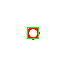
\begin{tikzpicture}
            \begin{axis}[hide axis, xmin=0, xmax=1, ymin=0, ymax=1] % to prevent warnings
                \addplot[color=-red]              (0,0); \label{leg:bgk}
                \addplot[color=black, mark=star9] (0,0); \label{leg:lbe}
                \addplot[color=red,   mark=o]     (0,0); \label{leg:kes}
                \addplot[color=green, mark=square](0,0); \label{leg:dsmc}
                \addplot[color=blue]              (0,0); \label{leg:asym}
            \end{axis}
        \end{tikzpicture}
    }%
    \centering
    \includegraphics{couette/integrated/shear}
    \caption{Зависимость сдвигового напряжения от числа Кнудсена. \(k=\Kn\sqrt\pi/2\), а \(P_{\NS xy}^*\)
        соответствует решению уравнений Навье"--~Стокса с граничными условиями без скольжения.
        Показаны решения модельного уравнения Крука"--~Веландера~\ref{leg:bgk},
        линеаризованного уравнения Больцмана~\ref{leg:lbe},
        КПИМДС~\ref{leg:kes}, ПСМ~\ref{leg:dsmc} и асимптотическое решение~\ref{leg:asym}.}
    \label{fig:couette:shear}
\end{figure}

Вычисляются профили первых тринадцати моментов функции распределения для различных чисел Кнудсена и Маха.
На рис.~\ref{fig:couette:profiles:qx} показано, как кривизна профиля продольного теплового потока
меняет знак по мере роста числа Маха. Рис.~\ref{fig:couette:profiles:Pzz}
демонстрирует степень анизотропичности тензора давлений \(P_{ij}\).
На рис.~\ref{fig:couette:shear} проводится сравнение полученных результатов с другими методами.
Все данные согласуются между собой в пределах точности
(положения~\ref{defpos:Couette_flow} и~\ref{defpos:asymptotic_verification}).

%%%%%%%%%%%%%%%%%%%%%%%%%%%%%%%%%%%%%%%%%%%%%%%%%%%%%%%%%%

\begin{figure}
    \centering
    \subbottom[уравнения КГФ с граничными условиями второго порядка]{%
        \includegraphics[width=.48\textwidth]{{{snit/contours/asym-0.01-temp}}}
        \label{fig:sone_bobylev:kn0.01:temp-kgf}}
    \subbottom[уравнение Больцмана]{%
        \includegraphics[width=.48\textwidth]{{{snit/contours/kes-0.01-temp}}}
        \label{fig:sone_bobylev:kn0.01:temp-be}}
    \caption{Изотермические линии для \(\Kn=0.01\)}
    \label{fig:sone_bobylev:kn0.01:temp}
\end{figure}

\begin{figure}
    \centering
    \subbottom[уравнения КГФ с граничными условиями второго порядка]{%
        \includegraphics[width=.48\textwidth]{{{snit/contours/asym-0.01-vel}}}
        \label{fig:sone_bobylev:kn0.01:flow-kgf}}
    \subbottom[уравнение Больцмана]{%
        \includegraphics[width=.48\textwidth]{{{snit/contours/kes-0.01-vel}}}
        \label{fig:sone_bobylev:kn0.01:flow-be}}
    \caption{Стационарное поле скоростей для \(\Kn=0.01\); изолинии соответствуют модулю.}
    \label{fig:sone_bobylev:kn0.01:flow}
\end{figure}

\begin{figure}
    \scalebox{0}{
        \begin{tikzpicture}
            \begin{axis}[hide axis, xmin=0, xmax=1, ymin=0, ymax=1] % to prevent warnings
                \addplot[color=gnuplot6, dotted](0,0);                      \label{leg:heat}
                \addplot[color=gnuplot1, dashed](0,0);                      \label{leg:asym0}
                \addplot[color=gnuplot2, dashdotted](0,0);                  \label{leg:asym1}
                \addplot[color=gnuplot4, solid](0,0);                       \label{leg:asym2}
                \addplot[color=gnuplot7, only marks, mark=o](0,0);          \label{leg:data1}
                \addplot[color=gnuplot7, only marks, mark=square](0,0);     \label{leg:data2}
                \addplot[color=gnuplot7, only marks, mark=triangle](0,0);   \label{leg:data3}
            \end{axis}
        \end{tikzpicture}
    }%
    \centering
    \subbottom{%
        \includegraphics[width=.48\textwidth]{snit/vs_kn/top_temp}
        \label{fig:sone_bobylev:topT}}
    \subbottom{%
        \includegraphics[width=.48\textwidth]{snit/vs_kn/bottom_flow}
        \label{fig:sone_bobylev:bottomU}}
    \hypersetup{hidelinks} % to prevent colorlinks
    \caption{
        Некоторые граничные интегралы в зависимости от числа Кнудсена, полученные разными методами:
        уравнение теплопроводности~\ref{leg:heat},
        уравнения КГФ с граничными условиями ведущего порядка (только тепловое скольжение)~\ref{leg:asym0},
        первого~\ref{leg:asym1} и второго~\ref{leg:asym2} порядков,
        уравнение Больцмана на равномерной сетке~\ref{leg:data1} и неравномерной~\ref{leg:data2}.
        Планка у~\ref{leg:data1} соответствует абсолютной погрешности \(3\cdot10^{-4}\) поля скорости.
    }
    \label{fig:sone_bobylev:comparison}
\end{figure}

Во \underline{второй части} рассматривается течение между пластинами с синусоидальным распределением температур.
На рис.~\ref{fig:sone_bobylev:kn0.01:temp} и~\ref{fig:sone_bobylev:kn0.01:flow} видно,
что при \(\Kn=0.01\) асимптотическое решение с хорошей точностью воспроизводит кинетическое решение,
полученное КПИМДС (положение~\ref{defpos:asymptotic_verification}).
На рис.~\ref{fig:sone_bobylev:comparison} видно, что такой результат достигнут, главным образом,
благодаря граничным условиям, учитывающим тепловое скольжение, скачки скорости и температуры первого порядка.
Сравниваются решения КПИМДС, полученные на различных скоростных сетках.

%%%%%%%%%%%%%%%%%%%%%%%%%%%%%%%%%%%%%%%%%%%%%%%%%%%%%%%%%%

\begin{figure}
    \centering
    \includegraphics[width=\textwidth]{kgf/noncoaxial/cylinder5}
    \caption{Поле скоростей \(u_{i1}\) между двумя некоаксиальными цилиндрами при \(T_1=1\) и \(T_2=5\);
        изолинии соответствуют модулю.}
    \label{fig:cylinders:velocity}
\end{figure}

\begin{figure}
    \centering
    \begin{minipage}{.48\textwidth}
        \includegraphics[width=\textwidth]{kgf/temper/U-tau-cylinders}
        \caption{Максимальное значение \(u_{i1}\) при \(d=0.5\).
            Пропорционально \(\tau^3\) при \(\tau\to0\) и \(\tau^{3/2}\) при \(\tau\to\infty\).}
        \label{fig:cylinders:maxU}
    \end{minipage}
    \hfill
    \begin{minipage}{.48\textwidth}
        \includegraphics[width=\textwidth]{kgf/force/terms-cylinder-inner}
        \caption{Профили компонент действующей силы \(F_{x2}\) вдоль поверхности внутреннего цилиндра
            в полярных координатах при \(d=0.5\) и \(\tau=4\).
            \(\phi = -\pi/2\) соответствует точке~\(x=d-1\), \(\phi = \pi/2\) соответствует точке~\(x=d+1\).}
        \label{fig:cylinders:terms_inner}
    \end{minipage}
\end{figure}

\begin{figure}
    \centering
    \subbottom[Пунктирные линии соответствуют линейной зависимости]{%
        \includegraphics[width=.48\textwidth]{kgf/force/forces}
        \label{fig:cylinders:force:total}}
    \subbottom[Пунктирные линии соответствуют линейной зависимости для сфер и степени \(3/2\) для цилиндров]{%
        \includegraphics[width=.48\textwidth]{kgf/force/forces-close}
        \label{fig:cylinders:force:inverse}}
    \caption{Сила притяжения между цилиндрами (сферами) в зависимости от расстояния между их осями \(d\).}
    \label{fig:cylinders:force}
\end{figure}

В \underline{третьей части} рассматривается течение газа между равномерно нагретыми
некоаксиальными цилиндрами и сферами в континуальном пределе.
На рис.~\ref{fig:cylinders:velocity} изображено \emph{нелинейное термострессовое течение},
возникающее между поверхностями с температурами \(T_1 = 1\) и \(T_2 = 1+\tau\).
Оси цилиндров смещены вдоль оси \(x\) на расстояние \(d\).
На рис.~\ref{fig:cylinders:maxU} показана зависимость силы течения от разницы температур,
а на рис.~\ref{fig:cylinders:terms_inner} распределение отдельных компонент действующей силы.

Сила взаимодействия между цилиндрами, оказывается, подобна электростатической (положение \ref{defpos:snit_forces}).
В частности, для степенного молекулярного потенциала (\(\Gamma_2=\gamma_2T^s\),
\(\Gamma_7=\Gamma_3'-\gamma_7T^{2s-1}\)) можно записать
\begin{equation*}
    p_0\oint_S F_{x2}\dd{S} = \varder[C]{d} (T_2^s-T_1^s)(T_2^{1+s}-T_1^{1+s}),
\end{equation*}
где \(C\) "--- аналог электрической ёмкости. Для цилиндров и сфер,~\autocite{Smythe1954}
\begin{equation*}
    C_\mathrm{cyl} \propto \frac1{\theta}, \:
    C_\mathrm{sph} \propto  \sum_{n=1}^\infty \frac{R_1 R_2 \sinh\theta} {R_2\sinh n\theta - R_1\sinh (n-1)\theta}, \quad
    \cosh\theta = \frac{R_1^2 + R_2^2 - d^2}{2 R_1 R_2}.
\end{equation*}
На рис.~\ref{fig:cylinders:force} показаны соответствующие силы, вычисленные из уравнений КГФ.

%%%%%%%%%%%%%%%%%%%%%%%%%%%%%%%%%%%%%%%%%%%%%%%%%%%%%%%%%%

\begin{figure}
    \centering
    \subbottom[уравнения КГФ с граничными условиями второго порядка]{%
        \includegraphics[width=.9\textwidth]{{{snit/elliptic/second-0.02-flow}}}
        \label{fig:elliptic:flow:second}}\\
    \subbottom[уравнение Больцмана]{%
        \includegraphics[width=.9\textwidth]{{{snit/elliptic/kes-0.02-flow}}}
        \label{fig:elliptic:flow:boltzmann}}
    \caption{Стационарное поле скоростей при \(\Kn=0.02\); изолинии соответствуют модулю.}
    \label{fig:elliptic:flow}
\end{figure}

В \underline{четвёртой части} рассматривается течение между коаксиальными эллиптическими цилиндрами,
нагретыми до температур \(T_0 = 1\) и \(T_1 = 5\).
На рис.~\ref{fig:elliptic:flow} можно сравнить решение уравнения Больцмана с асимптотическим.
На рис.~\ref{fig:elliptic:flow:second} отчётливо видны
а) нелинейное термострессовое течение \(\OO{\Kn}\) во всём объёме,
б) термострессовое скольжение \(\OO{\Kn^2}\) возле граничных поверхностей.
Однако в области, где градиент температуры сравним с \(\Kn^{-1}\), гидродинамическое описание неприменимо.

%%%%%%%%%%%%%%%%%%%%%%%%%%%%%%%%%%%%%%%%%%%%%%%%%%%%%%%%%%

\underline{\textbf{Приложение}} состоит из одной части.
Она содержит вывод одномерных интегральных уравнений Фредгольма из линеаризованного уравнения Больцмана
для газа твёрдых сфер, необходимых для вычисления транспортных коэффициентов \(\Gamma_8\), \(\Gamma_9\), \(\Gamma_{10}\)
(положение~\ref{defpos:transport_coeffs}).

В \underline{\textbf{заключении}} приведены основные выводы и рекомендации:
%% Согласно ГОСТ Р 7.0.11-2011:
%% 5.3.3 В заключении диссертации излагают итоги выполненного исследования, рекомендации, перспективы дальнейшей разработки темы.
%% 9.2.3 В заключении автореферата диссертации излагают итоги данного исследования, рекомендации и перспективы дальнейшей разработки темы.
\begin{enumerate}[wide]

%%% плюсы и минусы KПИМДС для неравномерных сеток
\item Обобщение KПИМДС для неравномерных сеток приводит к дополнительным вычислительным трудностям.
В частности, усложняется алгоритм консервативного проецирования в интеграле столкновений,
повышаются требования к мощности множества кубатурных точек,
что в целом приводит к увеличению вычислительных затрат.
Кроме того, на неравномерной сетке, в общем случае, снижается точность кубатур функций близких к максвелловским.
Тем не менее в настоящем исследовании на численных примерах продемонстрировано,
как в рамках KПИМДС неравномерная прямоугольная сетка позволяет достичь высокой точности и эффективности
а) для детального разрешения плоских кинетических слоёв,
б) для медленных, но сильно неизотермических течений.
Настоящая область применения метода значительно шире, включая
гиперзвуковые течения и задачи при очень больших числах Кнудсена.
Неравномерные сетки позволяют эффективно аппроксимировать
как большой объём скоростного пространства в первом случае,
так и высокие градиенты функции распределения во втором.

%%% сложности и направления развития KПИМДС для неравномерных сеток
\item Важной задачей математического анализа KПИМДС остаётся вопрос сходимости
и особенно влияния проекционного шаблона на её скорость.
Неравномерные сетки неизбежно приводят к отрицательным проекционным весам,
которые могут стать причиной аномальных численных флуктуаций решения.
Этот проблема требует детального анализа.

%%% польза асимптотического анализа
\item Асимптотическая теория уравнения Больцмана для малых чисел Кнудсена
играет важнейшую роль в моделировании разреженного газа.
С её помощью можно получить не только значения транспортных коэффициентов из знания молекулярного потенциала,
но также истинные граничные условия для гидродинамических уравнений и, что немаловажно,
позволяет корректно описать существенно неравновесное поведение газа в слое Кнудсена.
На численных примерах было показано, как использование граничных условий первого и второго порядка
позволяет улучшить точность и качество асимптотического решения.
В настоящем исследовании применение асимптотической теории оказалось ещё шире.
Главным образом, она послужила надёжным инструментом верификации численного метода решения уравнения Больцмана.
Кроме того, использование асимптотического решения в качестве начального приближения позволило
значительно ускорить решение стационарных задач с малыми числами Кнудсена.

%%% ограниченность асимптотического анализа
\item Гидродинамическое описание газа может оказаться некорректным на масштабах существенно больше длины свободного пробега,
если градиенты макроскопических величин в некоторых областях сравнимы с обратным числом Кнудсена.
Достоверно описать поведение газа в этих существенно неравновесных областях
возможно только в рамках кинетического подхода.
Подобная ситуация встречается во многих реальных задачах.
В настоящем исследовании было продемонстрировано кардинальное изменение картины
медленного неизотермического течения при больших градиентах температуры.

%%% прикладное значение медленных неизотермических течений
\item Медленные неизотермические течения представляют интерес в набирающей обороты индустрии МЭМС.
В настоящем исследовании показано, что численное решение уравнения Больцмана в континуальном пределе
сходится к решению уравнений КГФ с соответствующими граничными условиями,
которые, таким образом, верно учитывают влияние сильных температурных
неоднородностей на процессы переноса в слаборазреженном газе.

\end{enumerate}


%\newpage

\ifdefmacro{\microtypesetup}{\microtypesetup{protrusion=false}}{} % не рекомендуется применять пакет микротипографики к автоматически генерируемому списку литературы
\ifnumequal{\value{bibliosel}}{0}{% Встроенная реализация с загрузкой файла через движок bibtex8
  \renewcommand{\bibname}{\large \authorbibtitle}
  \nocite{*}
  \insertbiblioauthor           % Подключаем Bib-базы
  %\insertbiblioother   % !!! bibtex не умеет работать с несколькими библиографиями !!!
}{% Реализация пакетом biblatex через движок biber
  \ifnumgreater{\value{usefootcite}}{0}{
  \insertbiblioauthorcited      % Вывод процитированных в автореферате работ автора
  }{
  \insertbiblioauthor           % Вывод всех работ автора
%  \insertbiblioauthorgrouped    % Вывод всех работ автора, сгруппированных по источникам
%  \insertbiblioauthorimportant  % Вывод наиболее значимых работ автора (определяется в файле characteristic во второй section)
  \insertbiblioother            % Вывод списка литературы, на которую ссылались в тексте автореферата
  }
}
\ifdefmacro{\microtypesetup}{\microtypesetup{protrusion=true}}{}

